



\newcommand{\prgrmparunleft}{
    \mypagel{Circuit électrique : symboles et
        conventions générateur et
        récepteur.

        Comportement générateur ou
        récepteur d’un dipôle.}
}


\newcommand{\prgrmparun}{
    \mypage{
        \begin{itemize}
            \item Réaliser un circuit électrique à partir d’un schéma donné,
                  et inversement, les symboles étant fournis.
            \item  Représenter le branchement d’un ampèremètre, d’un
                  voltmètre et d’un système d’acquisition ou d’un oscilloscope sur un schéma électrique.
        \end{itemize}
    }
}



\newcommand{\prgrmpardeuxleft}{
    \mypagel{
        Tension électrique, intensité
        électrique.

        Grandeurs périodiques : valeur
        moyenne, valeur efficace,
        composante continue et
        composante alternative.

        Grandeurs sinusoïdales.
    }
}

\newcommand{\prgrmpardeux}{
    \mypage{
        \begin{itemize}
            \item  Visualiser, à l’aide d’un système d’acquisition, des
                  représentations temporelles d’une tension électrique
                  périodique, d’un courant électrique périodique dans un
                  circuit et en analyser les caractéristiques (période,
                  fréquence, composantes continue et alternative).
            \item  Choisir le réglage des appareils pour mesurer une valeur
                  moyenne ou une valeur efficace.
            \item  Mesurer la valeur moyenne d’une tension électrique,
                  d’une intensité électrique dans un circuit.
            \item  Mesurer la valeur efficace d’une tension électrique, d’une
                  intensité électrique dans un circuit.
        \end{itemize}
    }
}



\newcommand{\prgrmpartroisleft}{
    Loi des mailles, loi des nœuds.
}

\newcommand{\prgrmpartrois}{
    \mypage{
        \begin{itemize}
            \item Utiliser les conventions d’orientation permettant
                  d’algébriser tensions et intensités électriques.
            \item Utiliser la loi des nœuds et la loi des mailles dans un
                  circuit comportant trois mailles au plus.
        \end{itemize}
    }
}

\newcommand{\prgrmparquatreleft}{
    \mypagel{
        Puissance et énergie
        électriques.

        Comportement énergétique d’un
        dipôle.

        Loi d’Ohm. Effet Joule.
    }
}



\newcommand{\prgrmparquatre}{
    \mypage{
        \begin{itemize}
            \item Analyser les transferts d’énergie dans un circuit électrique,
                  à partir du signe de la puissance et de la convention choisie.
            \item Calculer la puissance moyenne et l’énergie électrique
                  mises en jeu sur une durée donnée dans le cas d’un récepteur
                  et d’un générateur électrique.
            \item Analyser le domaine de validité d’un modèle à partir d’un
                  ensemble de mesures (dipôles passifs résistifs).
            \item Mesurer la puissance moyenne et l’énergie électrique
                  transportée par une ligne électrique pendant une durée donnée.
        \end{itemize}
    }
}


\newcommand{\prgrmparcinqleft}{
    Sécurité électrique.
}


\newcommand{\prgrmparcinq}{
    \mypage{
        Adopter un comportement responsable et respecter les règles de sécurité
        électriques lors des manipulations.
    }
}


\newcommand{\mypage}[1]{
    \begin{minipage}[t]{0.6\textwidth}
        {#1}
    \end{minipage}
}


\newcommand{\mypagel}[1]{
    \begin{minipage}[t]{0.35\textwidth}
        {#1}
    \end{minipage}
}

%	\setlength{\arrayrulewidth}{0.5mm}
%	\setlength{\tabcolsep}{18pt}
\newcommand{\programme}{
    \renewcommand{\arraystretch}{2}
    \begin{center}
        \begin{tabular}{@{}|l|l|@{}}
            \multicolumn{2}{c}{Programme : Énergie électrique}   \\ \midrule

            \begin{minipage}[t]{0.3\textwidth}
                {Savoirs}\end{minipage} & \mypage{Savoirs-faire}     \\\midrule

            \prgrmparunleft                    & \prgrmparun     \\
            \prgrmpardeuxleft                  & \prgrmpardeux   \\
            \prgrmpartroisleft                 & \prgrmpartrois  \\
            \prgrmparquatreleft                & \prgrmparquatre \\
            \prgrmparcinqleft                  & \prgrmparcinq   \\

            % Énergie et puissance.                      & \prgrmpardeux  \\

            % \begin{minipage}[t]{0.3\textwidth}
            %     Les conversions et les chaînes
            %     énergétiques.

            %     Stockage de l’énergie.\end{minipage}       & \prgrmpartrois \\

            % \begin{minipage}[t]{0.3\textwidth}
            %     Principe de la conservation de l’énergie.
            %     Rendement\end{minipage}  & \prgrmparquatre                  \\

            % Ressource d’énergie dite « renouvelable ». & \prgrmparcinq  \\

            \bottomrule\end{tabular}
    \end{center}

}
\newcommand{\mybot}[2]{${#1}_{#2}$}

\newcommand{\exa}{
    \begin{center}
        Dans le circuit suivant, nommer les nœuds et les mailles.
        \vspace{5pt}

        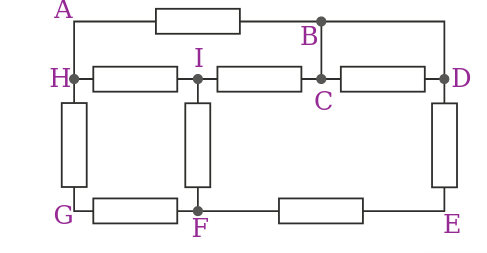
\includegraphics[width=0.8\columnwidth]{ex1.png}
    \end{center}
}

\newcommand{\exb}{
    \begin{center}
        Trouver une relation entre les différentes intensités.
        \vspace{10pt}

        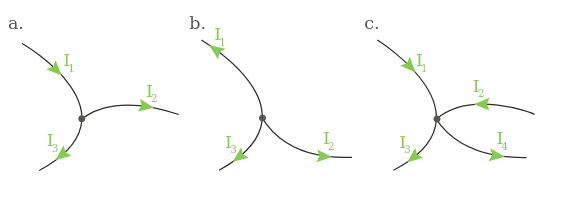
\includegraphics[width=1.2\columnwidth]{ex2.png}
    \end{center}
}

\newcommand{\exc}{

    On donne :
    \begin{center}
        \mybot{U}{AM} = 12 V ; \mybot{U}{AB}​= 2 V ; \mybot{U}{CD}= 1 V ; \mybot{U}{MD}= − 4 V;
    \end{center}
    \begin{itemize}
        \item Annoter sur le schéma les différentes tensions électriques (par exemple
              la tension aux bornes du générateur sera notée \mybot{U}{AM}.
        \item Établir les relations entre les tensions pour les mailles MABM et BCDMB.
        \item Calculer les valeurs des tensions \mybot{U}{BM} et \mybot{U}{BC}.
    \end{itemize}



    \begin{center}

        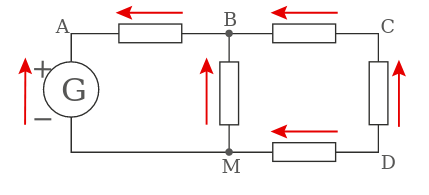
\includegraphics[width=0.8\columnwidth]{ex3.png}
    \end{center}
}
\newcommand{\exd}{


    Dans la maille (ABCDA)
    \begin{itemize}
        \item  Déterminer \mybot{U}{AD} en fonction des autres tensions de la maille.
        \item  Calculer \mybot{U}{AD} avec \mybot{U}{AB}= 2 V, \mybot{U}{BC}= 3 V et \mybot{U}{CD}= 4 V.
    \end{itemize}

    Dans la maille ADEA :
    \begin{itemize}
        \item  Déterminer \mybot{U}{ED} en fonction des autres tensions de la maille.
        \item  Calculer   \mybot{U}{ED} avec  \mybot{U}{EA}= 3 V.
    \end{itemize}

    \begin{center}
        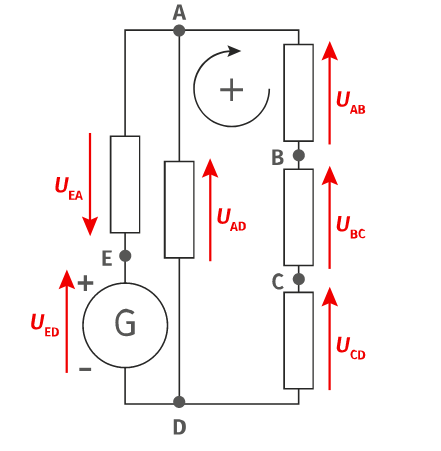
\includegraphics[width=0.6\columnwidth]{ex4.png}
    \end{center}

}
\newcommand{\exe}{
    \begin{center}
        1. Dans le circuit suivant, donner la relation existant entre les grandeurs $I_G​$, $I_1​$ et $I_2​$.

        2. Que deviennent les valeurs des intensités si l'ordre des dipôles dans la maille est changé ?

        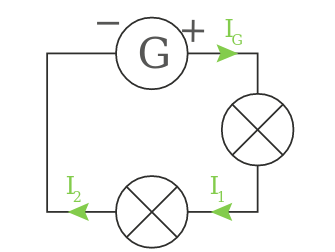
\includegraphics[width=0.7\columnwidth]{ex8.png}
    \end{center}


    % \begin{minipage}[c]{0.7\textwidth}
    %     1. Dans le circuit suivant, donner la relation existant entre les grandeurs IG​,I1​ et I2​.

    %     2. Que deviennent les valeurs des intensités si l'ordre des dipôles dans la maille est changé ?
    % \end{minipage}
    % % \hspace{0.1\textwidth}
    % \begin{minipage}[c]{0.35\textwidth}
    %     \begin{center}
    %         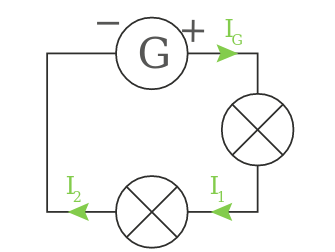
\includegraphics[width=0.6\columnwidth]{ex8.png}
    %     \end{center}
    % \end{minipage}


}

\newcommand{\exf}{
    \begin{center}
        Calculer la valeur de la résistance R en utilisant les relations existant entre les grandeurs tension et intensité.

        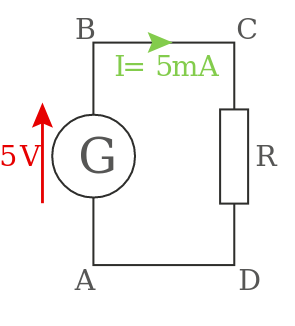
\includegraphics[width=0.5\columnwidth]{ex5.png}
    \end{center}
}

\newcommand{\exg}{
    \begin{center}

        Calculer la valeur de la résistance R. \vspace{2pt}

        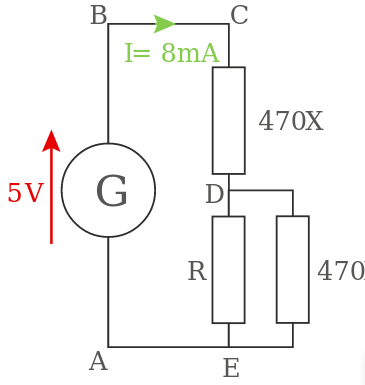
\includegraphics[width=0.6\columnwidth]{ex6.png}
    \end{center}
}

\newcommand{\exh}{
    \begin{center}

        Calculer la valeur de la résistance R.

        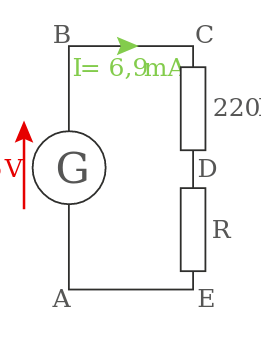
\includegraphics[width=0.6\columnwidth]{ex7.png}
    \end{center}

}
% \newcommand{\exi}{}
% \newcommand{\exj}{}
% \newcommand{\exk}{}
% \newcommand{\exl}{}
% \newcommand{\exm}{}
